\documentclass[]{scrartcl}

\usepackage{\string~"/LaTeX/StylePackage"}

\title{Biophysics Lab}
\author{Florian Bierlage}
\date{16.11.2024}


\begin{document}

\maketitle
\newpage
\tableofcontents
\newpage

\section{Introduction}

X-Rays, also called Röntgen Radiation, is a form of electromagnetic radiation with a wavelength of 10 nanometers to 10 picometers ($10^{-8}$ to $10^{-11}$ meters). This means that it has a smaller wavelength than Ultraviolet light, and with that the visible spectrum, meaning that it is not visible. X-Rays, unlike higher wavelength radiation, can penetrate material and interact with it on the subatomic level. In living organisms particularly this means that X-Rays interact with our cells, disrupting vital structures such as DNA. The body's cells either try to repair themselves, or if they are unrepairable they will self destruct. 

Cells undergo a continuous cell cycle, that is asexual reproduction, where they multiply their DNA and one cell will split into two.

\begin{center}
	\begin{figure}[h!]
	\includegraphics[width=8cm]{CellCycle}
	\caption{The Cell Cycle visualized, from Wikipedia}
	\end{figure}
\end{center}
Cells undergoing this cycle go through 5 phases. There is the $G_0$ phase, in which the cell is not actively dividing. The $G_1$ phase, in which the cell synthesized mRNA in preparation for the cell division, here there is also a \textit{Checkpoint}. The $S$ phase, in which the cell replicates its own DNA so that it has a copy of its own DNA. The $G_2$ phase in which the cell grows rapidly in preparation for Mitosis, this is another \textit{Checkpoint}. Lastly, there is the $M$ phase, which is Mitosis itself, the cell splits up into two separate cells with their own Organelles and their own copies of DNA, there is another \textit{Checkpoint} here.

The Checkpoints are very important. They are the points in which the Cell checks for DNA damage, meaning that the cell only halts growth in those given Checkpoints. The checkpoints occur when the Cell has one times its own DNA, two times its own DNA and when it's going through Mitosis

This experiment serves to research how different radiation doses harm cells, both short term and long term effects. In addition, despite already knowing where the Checkpoints are beforehand, we will re-confirm this fact.
\newpage
\section{Methods}

After irradiation cells within the cell cycle will go through the checkpoints $G_1$, $G_2$ and $M$, and will halt growth. We will measure the DNA inside the cells to check how many Cells are in which Checkpoint. We will do this by use of Flow Cytometry, by measuring the amount of DNA in the cells, as cells in the $G_2$ checkpoint have twice the DNA as cells in the $G_1$ checkpoint.

Flow Cytometry works by shining a laser through the cells one by one, which then reflect it or shine in fluorescence. Importantly, the cells that are fed through the flow cytometer first need to be prepared. Here, the cells are soaked in propidium iodide (PI) which binds to DNA, and gives off Fluorescent light.

Before doing this the cells are soaked in Ribonuclease which breaks down the RNA inside the cell. This is done because the PI does not only bind to DNA but also to RNA, and it would lead to inaccuracies in the measurements.
\begin{center}
	\begin{figure}[h!]
	\includegraphics[width=11.5cm]{FlowCytometer}
	\caption{An Image describing the flow cytometer process from Streck.com}
	\end{figure}
\end{center}
The data will only be from the light that is fluoresced by the PI, as it will be the data representing the amount of DNA inside the Cell. This process is done with Cells that have not been irradiated, cells that have gotten a dose of $0.5 Gy$ and cells that have gotten a dose of $5 Gy$. This will facilitate a comparison of how DNA is distributed for healthy cells and how low and high radiation doses affect this distribution. 

The healthy cells should present mainly cells with one times their DNA, and then an even distribution of cells that have anywhere between one times and two times their DNA. As the cells do not accumulate at any checkpoints we should expect cells to be distributed according to how long the phase of the cell cycle takes.

The irradiated cells should present cells that have clearly halted progress in the checkpoints. This means that there should be a peak for every checkpoint, with a smaller distribution of healthy cells that are still undergoing the cell cycle, so the peaks should be higher in comparison to the general distribution that was shown in the healthy cells.

\subsection{Procedure}

The procedure for the observation of immediate effects of radiation is simple. The unirradiated cells are taken and Irradiated with doses of $0.5Gy$ and $5Gy$. Afterwards they are put back to incubate, and then they can be observed under a microscope.\\
The long-term effect cell groups need to be prepared a day in advance.

On the preparation day: The cell groups are irradiated and then left to incubate for 5 hours. two groups are irradiated at $5Gy$, two are irradiated at $0.5Gy$, and two aren't irradiated at all as control groups. The X-Ray is operated at $220kV$\\
After Incubation the cells are Trypsinized and centrifuged. This is done so that the cells are separated for the flow cytometry. After that they are rinsed twice with PBS and centrifuged again to remove the Trypsin.\\
Then they are prepared for Refrigeration. Suspend the cells in PBS and vortex them, to distribute them evenly in the liquid. Add ethanol to the mixture in drops. This helps fix the cells so that they do not degrade while being refrigerated. The cells are then Refrigerated for 24 to 48 hours or longer at -20 degrees Celsius

On the day of the experiment: The cell samples are centrifuged. The excess liquid is removed. PBS is added, the cells are centrifuged and the excess liquid is removed twice again. The cells are then suspended in a solution of PBS, PI and RNase.\\
The samples are then Incubated for 45 minutes, afterwards filtered and run through the flow cytometer.


\newpage
\section{Results}

To see the immediate effects of Radiation, unirradiated cells were compared against cells that had been irradiated with 0.5$Gy$ and $5Gy$. This was done under a microscope. The difference between $0.5 Gy$ and the control group was not very big, however it was noticable that the $5Gy$ group had a lot more dead cells, which points to cells killing themselves immediately if they get a sufficient radiation dose.

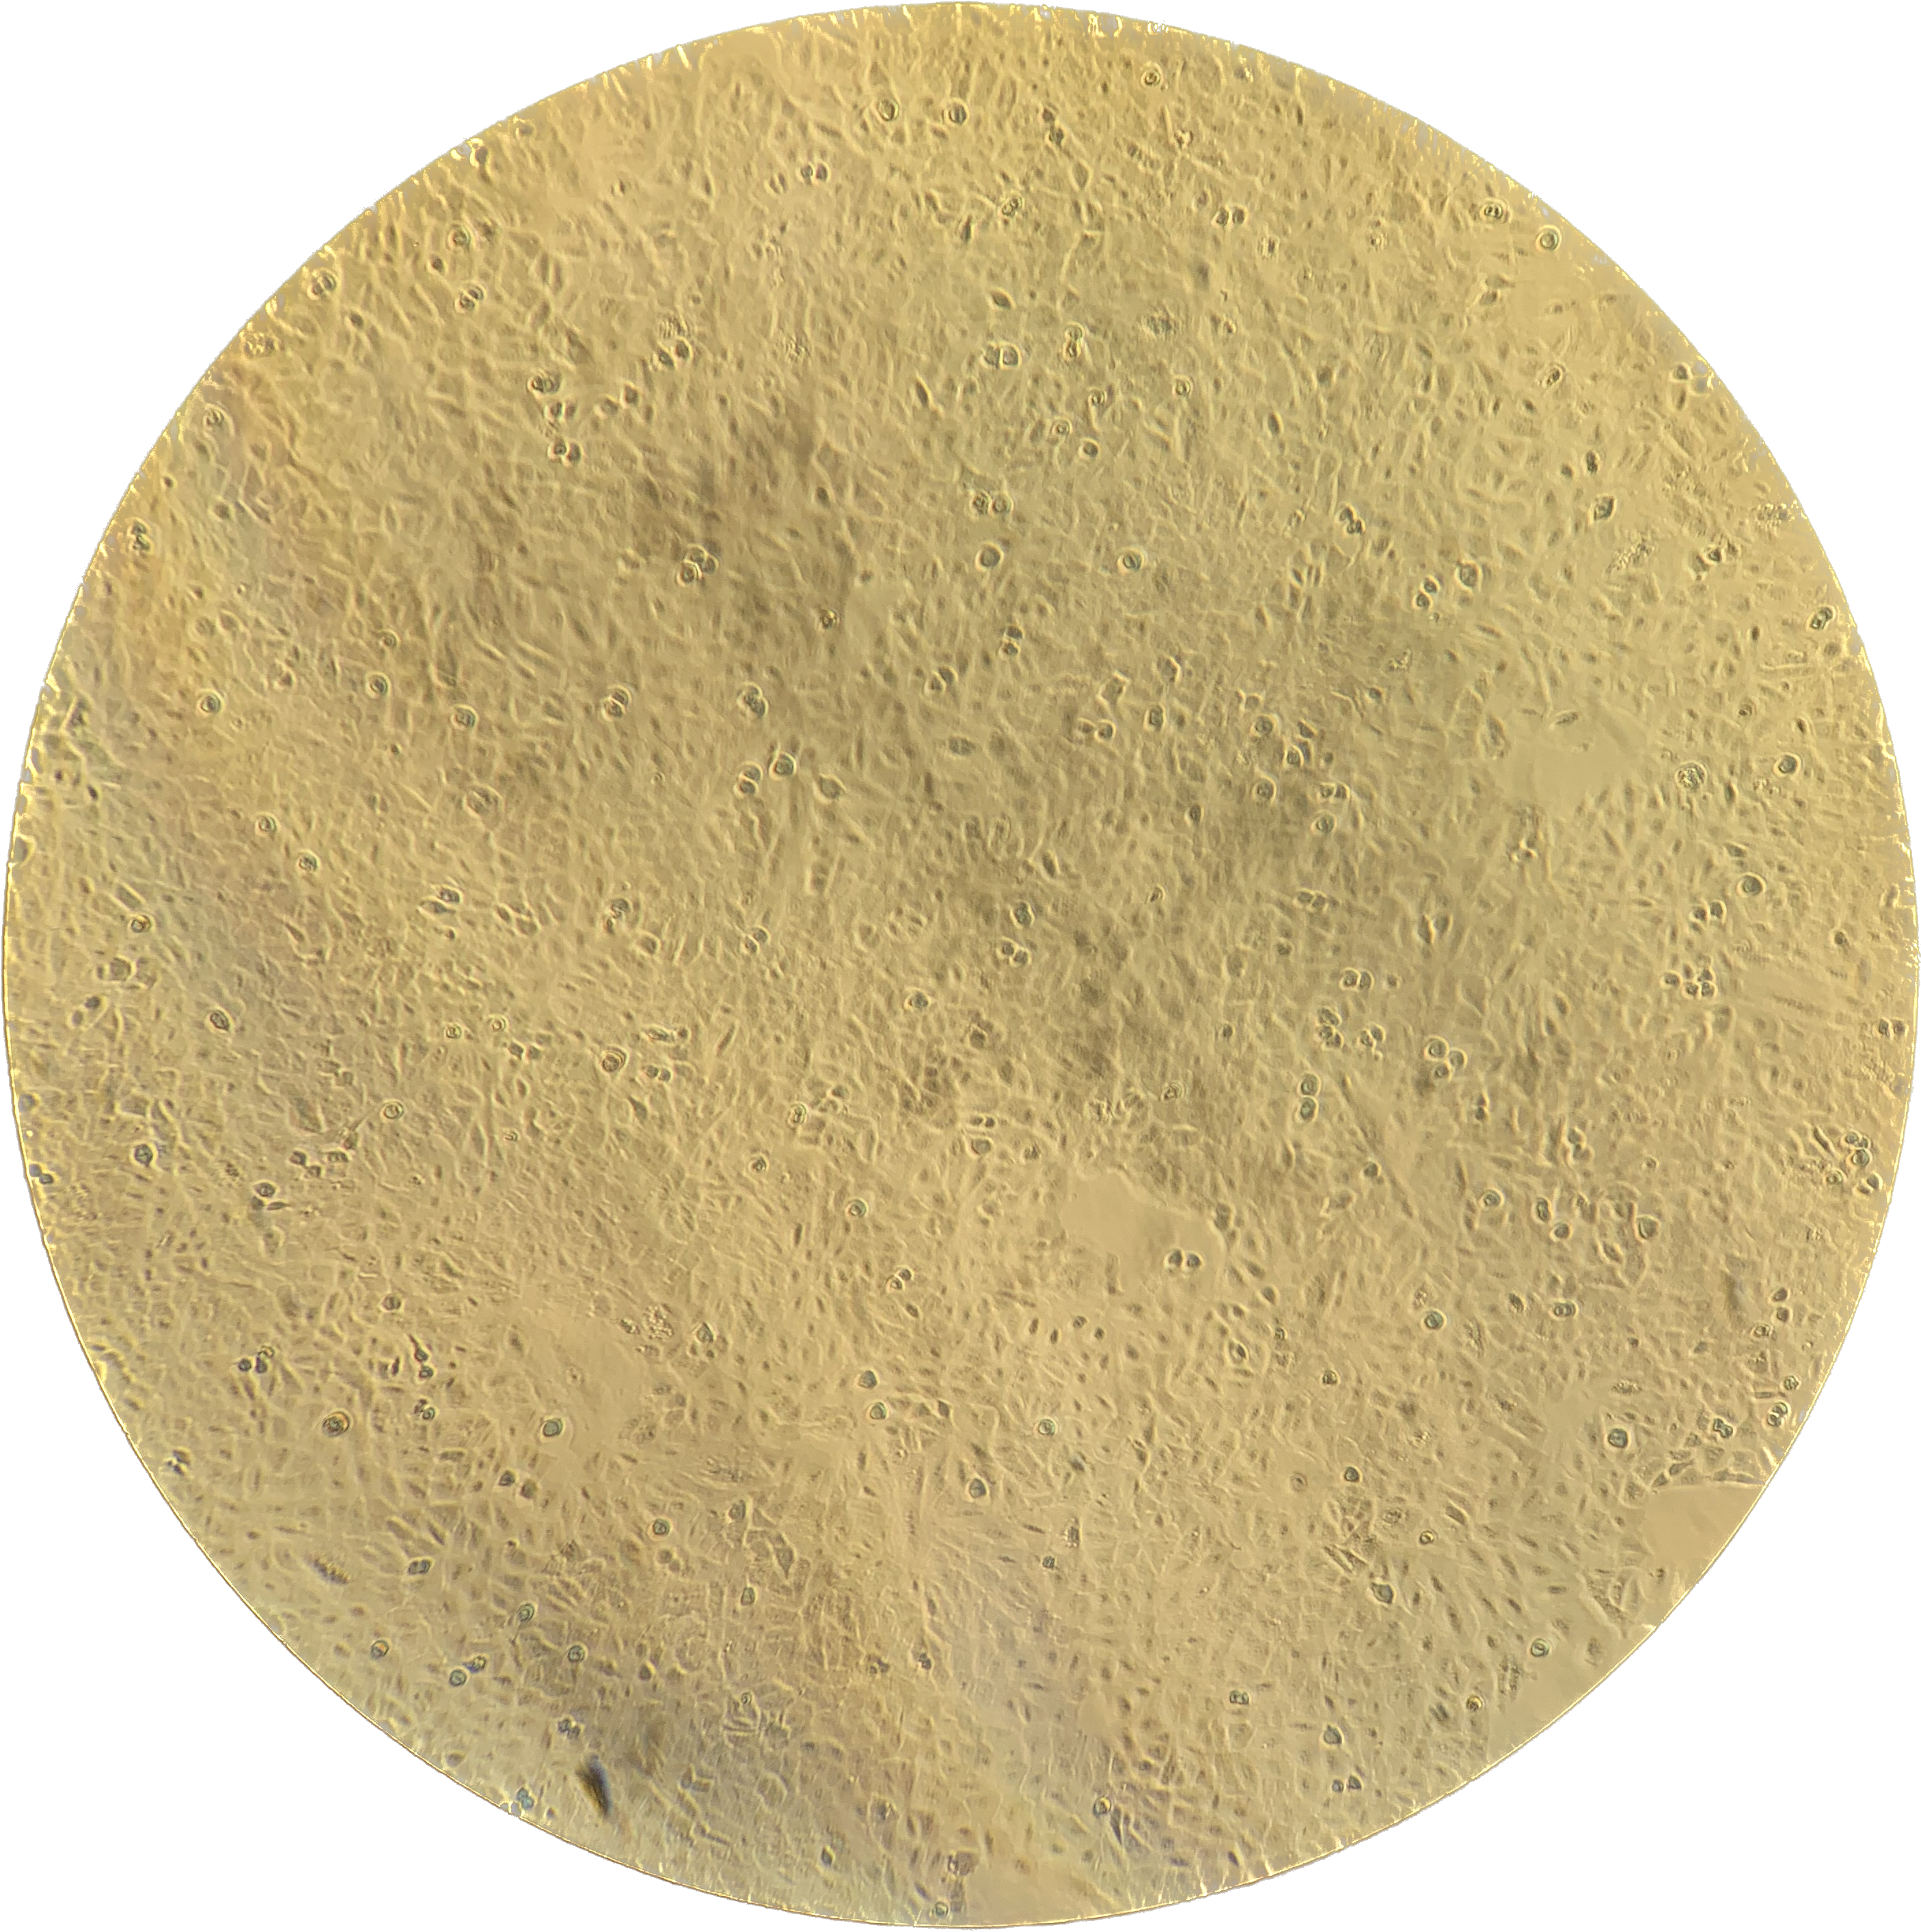
\includegraphics[width=13cm]{MicroscopeImage}

This is an image of the irradiated cells, the dead cells are visible as out of focus blots, while the live cells are highly in contrast. There are some cells visible that appear to stick together, these are cells that are in the middle of splitting. This demonstrates that splitting cells don't immediately self destruct when irradiated.

\newpage

For the long-term effects of Radiation the flow-cytometry data has been collected in histograms, where the fluorescent light that every cell gave off was recorded.

\begin{center}
\begin{figure}[h]
	\begin{subfigure}{0.5\textwidth}
		\includegraphics[width=\linewidth]{Zero}
	\end{subfigure}
	\begin{subfigure}{0.5\textwidth}
		\includegraphics[width=\linewidth]{pointfive}
	\end{subfigure}
\end{figure}
\end{center}
\begin{center}
\includegraphics[width=13cm]{five}
\end{center}
From the histogram of the unirradiated cells it is quite clear that the Cells that have one times or two times their DNA lie at about 700 and 1400 units. Therefore the range 600-800 will be counted as one times DNA and the range 1300-1500 will be counted as two times DNA. Then we get the following Data:
\begin{center}
	\begin{tabular}{|c||c|c|c|}
		\hline
		& once & twice & $\frac{\text{twice}}{\text{once}}$\\ \hline\hline
		$0.5Gy$ & 19900 & 2800 & 14\% \\
		$5Gy$ & 13300 & 5600 & 42\% \\
		$0Gy$ & 6200 & 600 & 9\% \\
		\hline
	\end{tabular}
\end{center}
This shows that the higher the dose the more cells will have twice their DNA. This demonstrates the $G_2$ checkpoint. Additionally, there are less cells going from the one time DNA state to the two times DNA state, showing the $G_1$ checkpoint. However, it is important that the $G_1$ checkpoint is not as strong as the $G_2$ checkpoint, which results in cells still being able to go through the cell cycle and then stopping at the $G_2$ checkpoint.

In the Histogram for the $5Gy$ dosis there are also many cells which lie outside the bound of one or two times their DNA. This is probably due to imprecise filtering, which caused more faulty cells to be analyzed in the flow cytometer.


\section{Discussion}
This experiment has clearly shown the harm of X-Rays to cells. 

There are immediate effects, which causes cells to self destruct in order to prevent mutation, with a higher radiation dose resulting in a higher percentage of cells dying.

There are also long-term effects, in which cells halt their cell cycles in order to assess damages. This results in the identification of two checkpoints via flow cytometry, that being the $G_1$ and $G_2$ checkpoints. It is also visible that the $G_1$ checkpoint isn't as strong as the $G_2$ checkpoint, as there are still many cells that go from the $G_1$ phase to the $S$ phase, however with increasing doses there are less cells that do this.


\end{document}

